\chapter{Diseño de un chatbot de ayuda a la terapia de reminiscencia}
\label{cap:ChatBot final}
Este capítulo tiene como objetivo presentar la solución final desarrollada a partir de la problemática presentada en el capítulo \ref{sec:objetivos}. Para ello, se describirá en profundidad cada uno de los componentes básicos de la arquitectura del sistema, y se presentara esta en sí misma. Por otro lado, se explicará tanto el proceso de puesta en marcha como las herramientas necesarias para ese mismo objetivo. 

Con el objetivo de permitir la opción de estudiar los componentes de forma práctica, es decir, usando el prototipo, este capítulo comenzará por la explicación de la puesta en marcha. A continuación, se dará una idea global de la arquitectura del sistema y finalmente se irá explorando en cada sección, cada uno de los módulos que la componen. 
\section{Herramientas y puesta en marcha}
Para la puesta en marcha el primer paso es obtener la \textit{API Key} para lo que es necesario el uso de una VPN.
\subsection{VPN}
Debido a las restricciones geográficas actuales de la API de Gemini para poder usarla es necesario el uso de una VPN. En concreto y para el desarrollo de este proyecto la conexión a la VPN se ha realizado mediante la herramienta \textit{hide.me VPN}. Esta herramienta crea un túnel seguro utilizando protocolos VPN, oculta nuestra IP real con una suya y cifra todo el tráfico de internet que pasa por este túnel para que podamos navegar libremente. Además, \textit{hide.me} está certificada como una VPN cero registros. Esto significa que no se almacena información de ningún tipo. El uso de la VPN es necesario tanto para obtener la \textit{API Key} como para el uso de la misma. Los países en los que se encuentra disponible gemini se pueden consultar en la web \href{https://ai.google.dev/gemini-api/docs/available-regions?hl=es-419} de la api de gemini. 

\subsection{Instalación de la API de Gemini}

Para comenzar a utilizar la API de Gemini con Python, es necesario seguir estos pasos para instalar el SDK y configurar tu clave de API.

En primer lugar, instalamos el SDK \footnote{\url{https://ai.google/discover/generativeai/}} (Software Development Kit). La API de Gemini está contenida en el paquete \texttt{google-generativeai} \footnote{\url{https://ai.google.dev/gemini-api/docs/available-regions?hl=es-419}} en PyPI, por lo que el primer paso sera instalar esa dependencia.

\begin{lstlisting}[language=Python]
	!pip install -U google-generativeai
\end{lstlisting}

Para utilizar la API de Gemini, se necesita una clave de API obtenida del \href{https://aistudio.google.com/app/apikey} Google AI Studio. Una vez que tengas tu clave, puedes configurarla para que el SDK la utilice:

\begin{lstlisting}[language=Python]
	import google.generativeai as genai
	from google.colab import userdata
	
	GOOGLE_API_KEY = userdata.get('GOOGLE_API_KEY')
	genai.configure(api_key=GOOGLE_API_KEY)
\end{lstlisting}


Siguiendo con la arquitectura del sistema bastaría con modificar en el archivo \textit{config.py} el valor de la \textit{API KEY}.

\subsection{Puesta en marcha} 
Una vez hechas todas las configuraciones necesarias explicadas en las secciones anteriores, para poder usar el chatbot sería necesario poner en ejecución el módulo $mibot.py$ y enviar el comando $\backslash start$ al usuario $\makeatletter @ mavice07\_bot$. Es importante recordar, que para que el análisis de la información y el flujo de la conversación se desarrollen correctamente, hay que estar conectado a una VPN de una de las localizaciones en las que se encuentra disponible la API de gemini, y que como ya se ha comentado con anterioridad, se pueden consultar en \href{https://ai.google.dev/gemini-api/docs/available-regions?hl=es-419} la web de Gemini.
\section{Arquitectura del sistema}
Con todo lo implementado, el sistema se puede representar como se ve en la figura \ref{fig:arquitectura}. 

\begin{figure}[h]
	\centering
	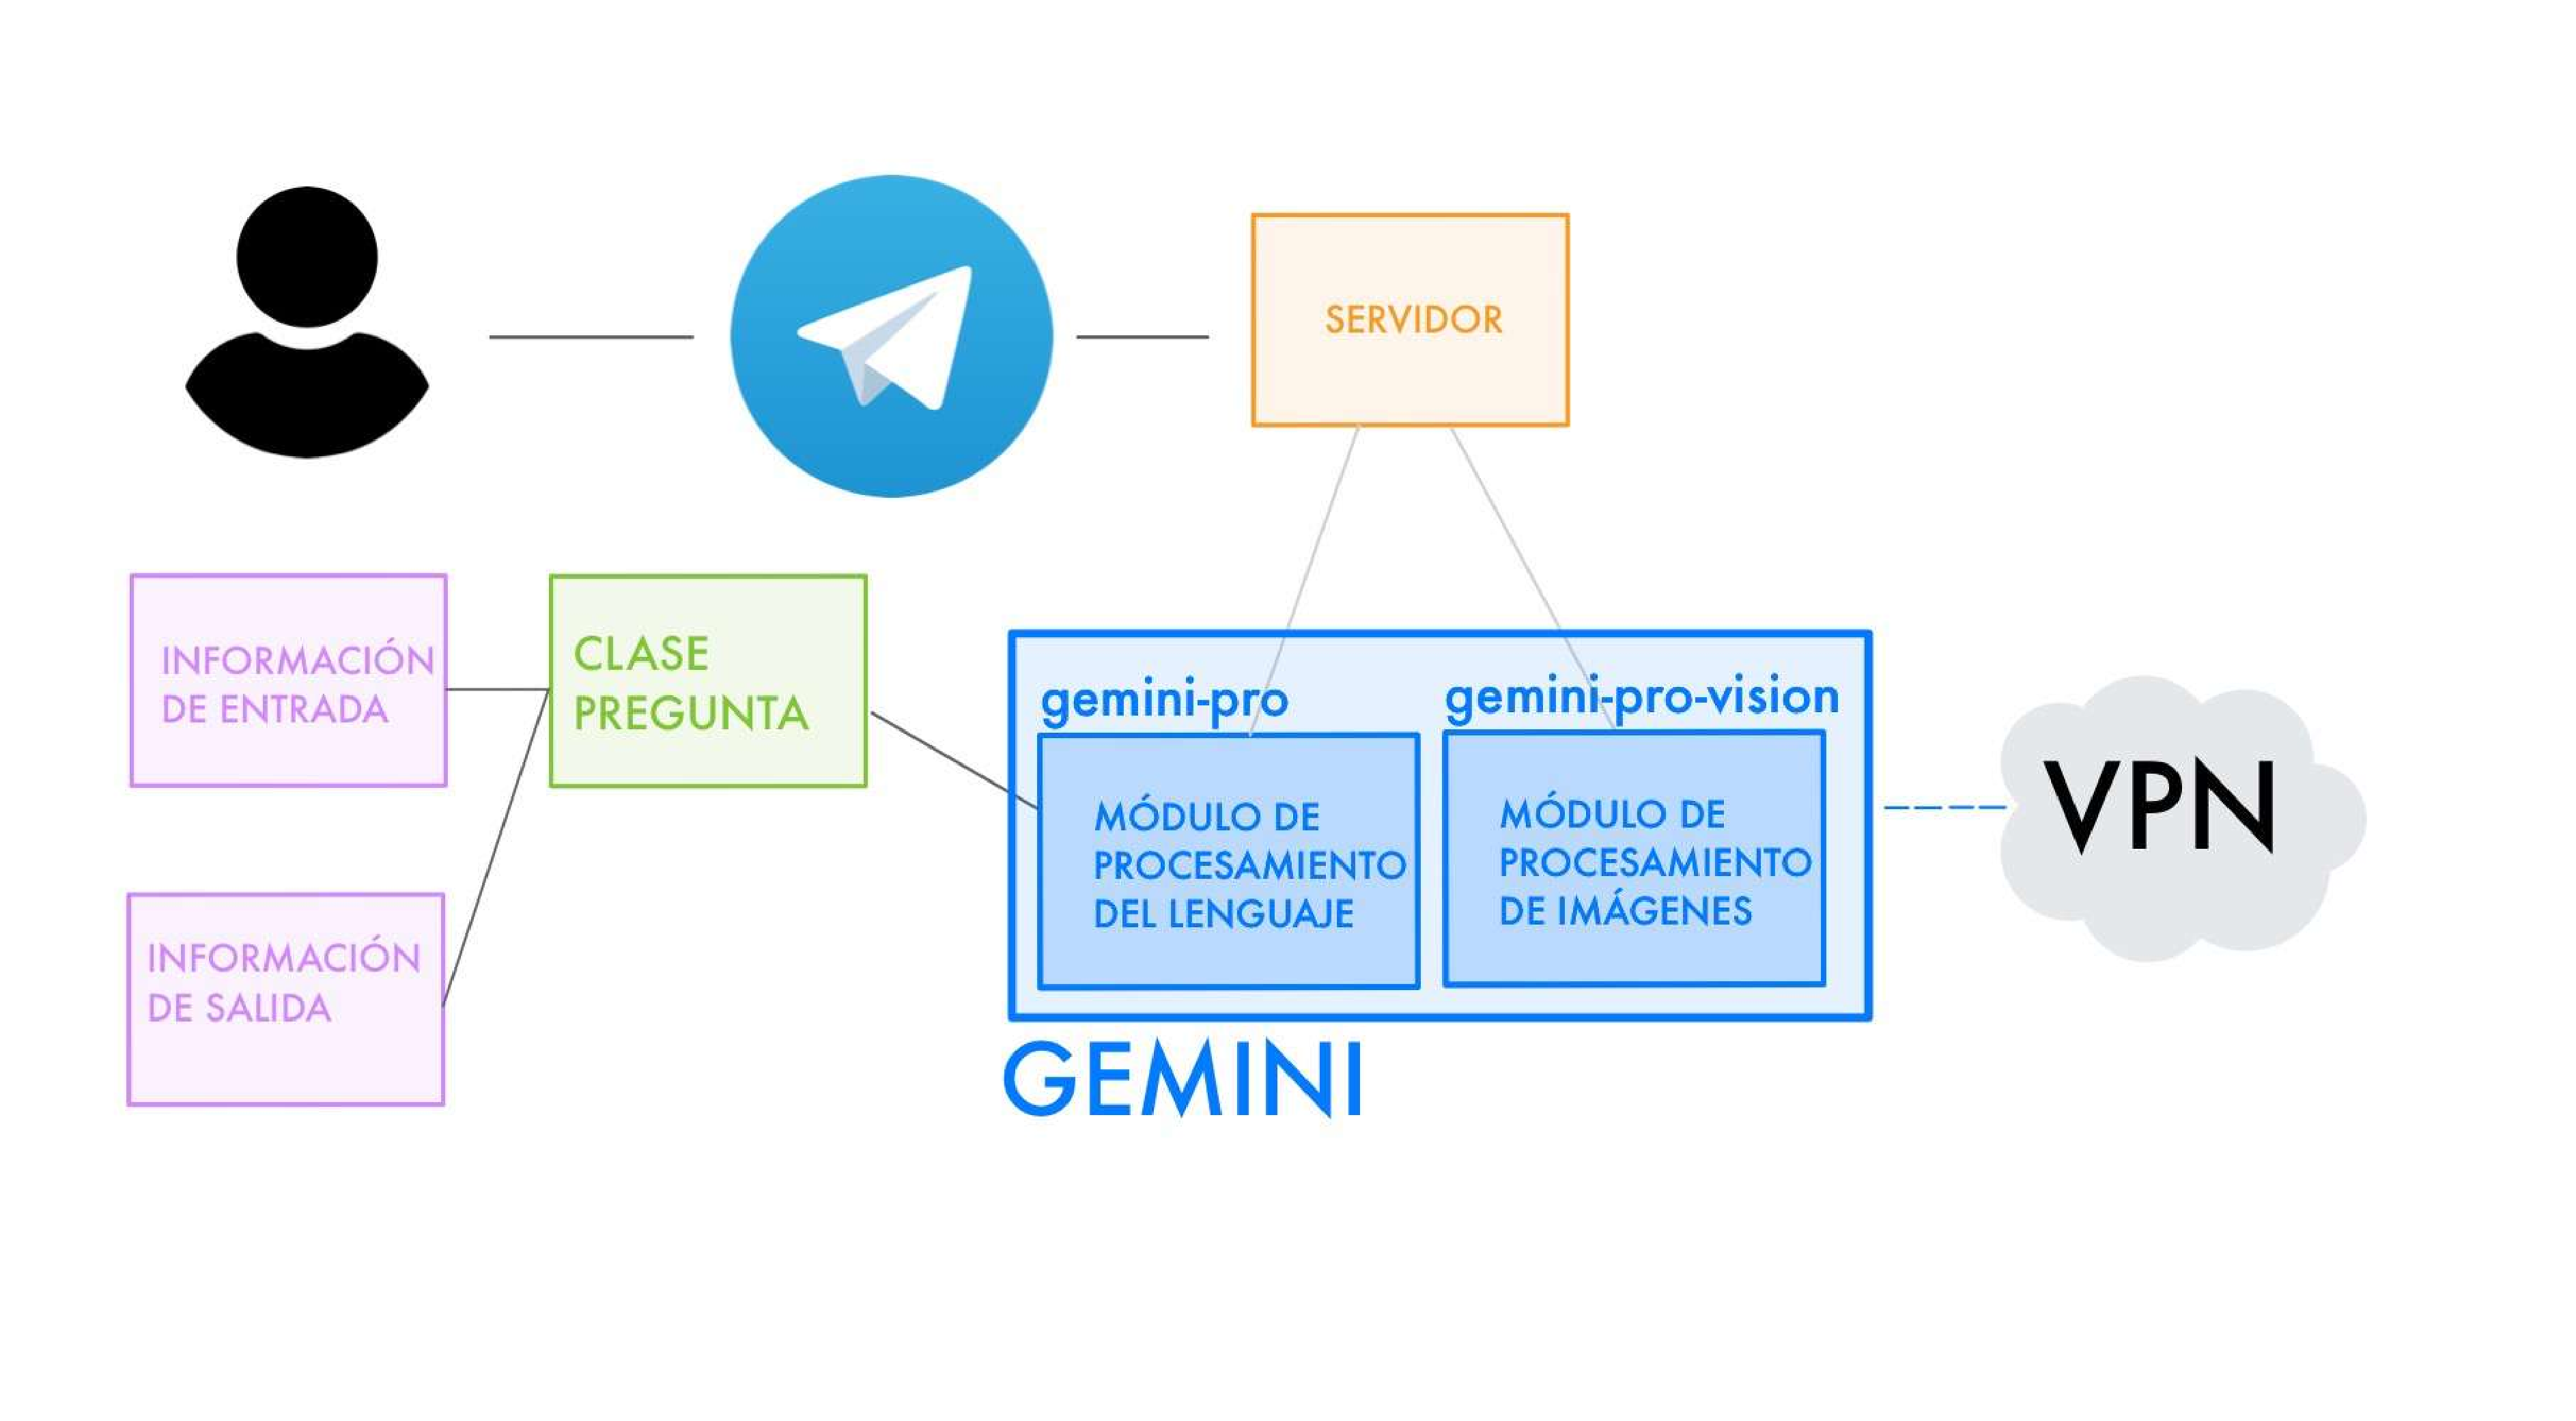
\includegraphics[width=1\textwidth]{Imagenes/arquitectura}
	\caption{Arquitectura del sistema}
	\label{fig:arquitectura}
\end{figure}

\subsection{Servidor}

El módulo servidor se encarga de manejar el flujo de los mensajes del chatbot. Recibe los mensajes entrantes desde la plataforma de Telegram y coordina su procesamiento posterior. Este módulo actúa como el punto de entrada centralizado del sistema, y ha de mantenerse en ejecución durante todo el tiempo en el que se quiera usar el chatbot.

La lógica del módulo para manejar los mensajes sigue lo explicado en la sección \ref{sec:Telegram}.  Esta capacidad de coordinación del módulo servidor asegura una distribución eficiente de los mensajes entrantes optimizando así la velocidad de respuesta y la efectividad de las interacciones con los usuarios. Este manejo eficiente se hace a través del uso de tres manejadores, cada uno encargado de gestionar los tres tipos de mensajes de entrada: comandos, imagenes y texto. 


\begin{itemize}
	\item El manejador $cmd\_start()$ se activa únicamente cuando un usuario envía el comando $\backslash start$ al bot. Este manejador inicia la lógica del bot al cargar las preguntas utilizando la función $cargar\_preguntas()$ del módulo $tfg$ y envía un mensaje de bienvenida al usuario.
	
	\item El manejador $bot\_mensajes\_text()$ se activa cuando un usuario envía un mensaje de texto al bot. Si el mensaje comienza con "$\backslash$", se envía un mensaje de error indicando que el comando no está disponible. Si es un mensaje de texto estándar, se llama a la función $siguientePregunta()$ del módulo $tfg$ y se analiza el mensaje como respuesta al último mensaje enviado por el bot. De esta forma se procesa la respuesta del usuario y se genera una respuesta apropiada.
	
	\item El manejador $photo()$ se activa cuando un usuario envía una foto al bot. El manejador descarga la foto y la guarda en el sistema de archivos. A continuación, llama a la función $analizador\_imagenes()$ del módulo $imagenes$ para analizar la imagen y generar una respuesta apropiada. El modelo de \textit{gemini-pro-vision} carga la foto descargada y la analiza con el prompt que le indica que describa la imagen y genere una pregunta. 
\end{itemize}

El módulo servidor sirve como el núcleo activo del chatbot, recibiendo mensajes desde Telegram y dirigiéndolos hacia los componentes adecuados del sistema para su procesamiento y respuesta. Su función es fundamental para mantener el flujo de comunicación entre los usuarios y el chatbot, facilitando una experiencia de usuario fluida y receptiva. 

\subsection{Módulo de procesamiento del lenguaje}
El módulo del procesamiento de la información es el que usa Gemini, y que por tanto requiere estar conectado a una VPN. En función del tipo de mensaje de entrada, imagen o texto, el servidor enviará la información al módulo de procesamiento del lenguaje o al módulo del procesamiento de imagenes.

Cuando se ha iniciado el chatbot y se han cargado las preguntas, el resto de mensajes de texto serán analizados por este módulo. La tarea principal del módulo es ir pasando una por una por todas las preguntas predefinidas rellenando la información y almacenando las respuestas. 

Cuando el módulo hace una pregunta, almacena la respuesta y la manda a analizar con los prompts y funciones ya explicadas en la sección \ref{protogemini}. Estas funciones se encargan de coger la respuesta del usuario , extraer la información útil y asociarla a campos predefinidos (además de añadir nuevos campos si hay información extra).

El manejo de la información se lleva a cabo a través de ficheros. Cuando el servidor recibe el comando $\backslash start$ carga y crea las preguntas del fichero \textit{preguntas.txt}. Una vez llevada a cabo toda la conversación con el usuario, la información obtenida y la información generada se guardan en el fichero de salida \textit{información.txt}

En el módulo de procesamiento de texto se agrupa la mayoría de la funcionalidad del chatbot. Para entender mejor cuál es el flujo de la información vamos a ver las diferentes tareas que realiza a través de un ejemplo concreto. 

\begin{itemize}
	\item Control de la lógica del sistema y flujo de las preguntas.
	
	 Cuando empieza la conversación el módulo se encarga de cargar toda la información a partir del fichero \textit{preguntas.txt} y transformarla en objetos de la clase ``Pregunta''. A continuación, se encarga de manejar el flujo de la conversación a través de las preguntas predefinidas que acaba de cargar. Supongamos que nos encontramos en plena conversación y que se ha lanzado al usuario la pregunta ``¿Cuáles son tu comida y bebida favoritas?'' con campos asociados ['comida favorita', 'bebida favorita']. Hemos obtenido la respuesta ''Mi comida favorita son las lentejas pero detesto los garbanzos''.
	
	\item Análisis de las respuestas.
	
	 Una vez recibida la respuesta esta pasaría a ser analizada. Si llamamos al modelo usando los prompts indicados en \ref{analisisres} obtenemos la siguiente respuesta. 
\begin{verbatim}
'```json\n{\n  "comida favorita": [\n    "Lentejas"\n  ],\n  "bebida
	 favorita": [\n    "No Encontrado"\n  ], \n "comida detestada":[\n
	  garbanzos]\n}\n```'
\end{verbatim}

La información se extrae de forma adecuada, e incluso se añade información adicional que no se corresponde con ningún campo predefinido. Esto ocurre gracias a una llamada adicional al modelo en la que se pide que añada información extra en caso de haberla encontrado, como se explica en \ref{analisisres}

	\item Generación de los \textit{json} con la información.

El siguiente paso es enviar este valor a diferentes funciones que se encargan en transformar ese \textit{string} en el suguiente \textit{json}, que se almacena en el atributo \textit{campos} del objeto ``Pregunta'' asociado. 
\begin{verbatim}
{'comida favorita': ['lentejas'], 'bebida favorita': ['No Encontrado'],
	 'comida detestada': ['garbanzos']}
\end{verbatim}

	\item Identificación de la información ausente.
	
	 Cuando termina la fase de extracción de la información y se ha generado el \textit{json} resulta sencillo comprobar para que campos no se ha obtenido información. Antes de pasar a la siguiente pregunta predefinida, se itera sobre todos los campos comprobando que no hay información ausente. En caso de encontrar un campo para el que no se ha encontrado valor. Se pasa a la etapa de generación de preguntas. 
	
	\item Generación de preguntas adicionales.
	
	 Como se puede ver, en nuestro caso no se ha obtenido información para el campo ``bebida favorita'' con lo que se generan preguntas para este campo como se explica en la sección \ref{generacionpreguntas}. Con esto se actualiza el atributo ``Preguntas extra'' del objeto ``Pregunta'' y se pasa a ir realizando estas preguntas una a una hasta que se rellene el campo ``bebida favorita'' o hasta que se acaben las preguntas extra generadas. En este segundo caso, no se generaran más preguntas si no que se pasará a continuar con el flujo normal de la conversación. 
	
	Igual que ocurría con la extracción de información, la respuesta que da \textit{gemini} necesita ser parseada para obtener las respuestas con un formato ``limpio''. Un ejemplo de generación de preguntas para el campo ``bebida favorita''. Supongamos que en la lista de preguntas generadas se encuentra la siguiente, y que al hacérsela al usuario se obtiene la respuesta mostrada a continuación. 
	
\begin{verbatim}
¿Cuál es tu bebida favorita? 
>>> Mi bebida favorita es el café, pero de jovén me gustaba la
 cerveza.

\end{verbatim}

Esta pregunta y respuesta se almacenarían en el diccionario ``respuestasExtra'' y se analizarían según lo explicado anteriormente como una respuesta normal. Tras todo el proceso de extracción de la información el atributo campos queda como sigue. 

\begin{verbatim}
{'comida favorita': ['lentejas'], 'bebida favorita': ['café'], 
	'comida detestada': ['garbanzos'], 'bebida juventud' : ['cerveza'] }

\end{verbatim}
	 \item Generación de feedback a las respuestas del usuario.
	 
	  Para tener una sensación de conversación más real y que el chatbot no se limite sólo a hacer preguntas, se le pide al modelo que genere cierto feedback para las respuestas. Por ejemplo, como se muestra en la figura \ref{fig:feedback}.
\end{itemize}

\begin{figure}[h]
	\centering
	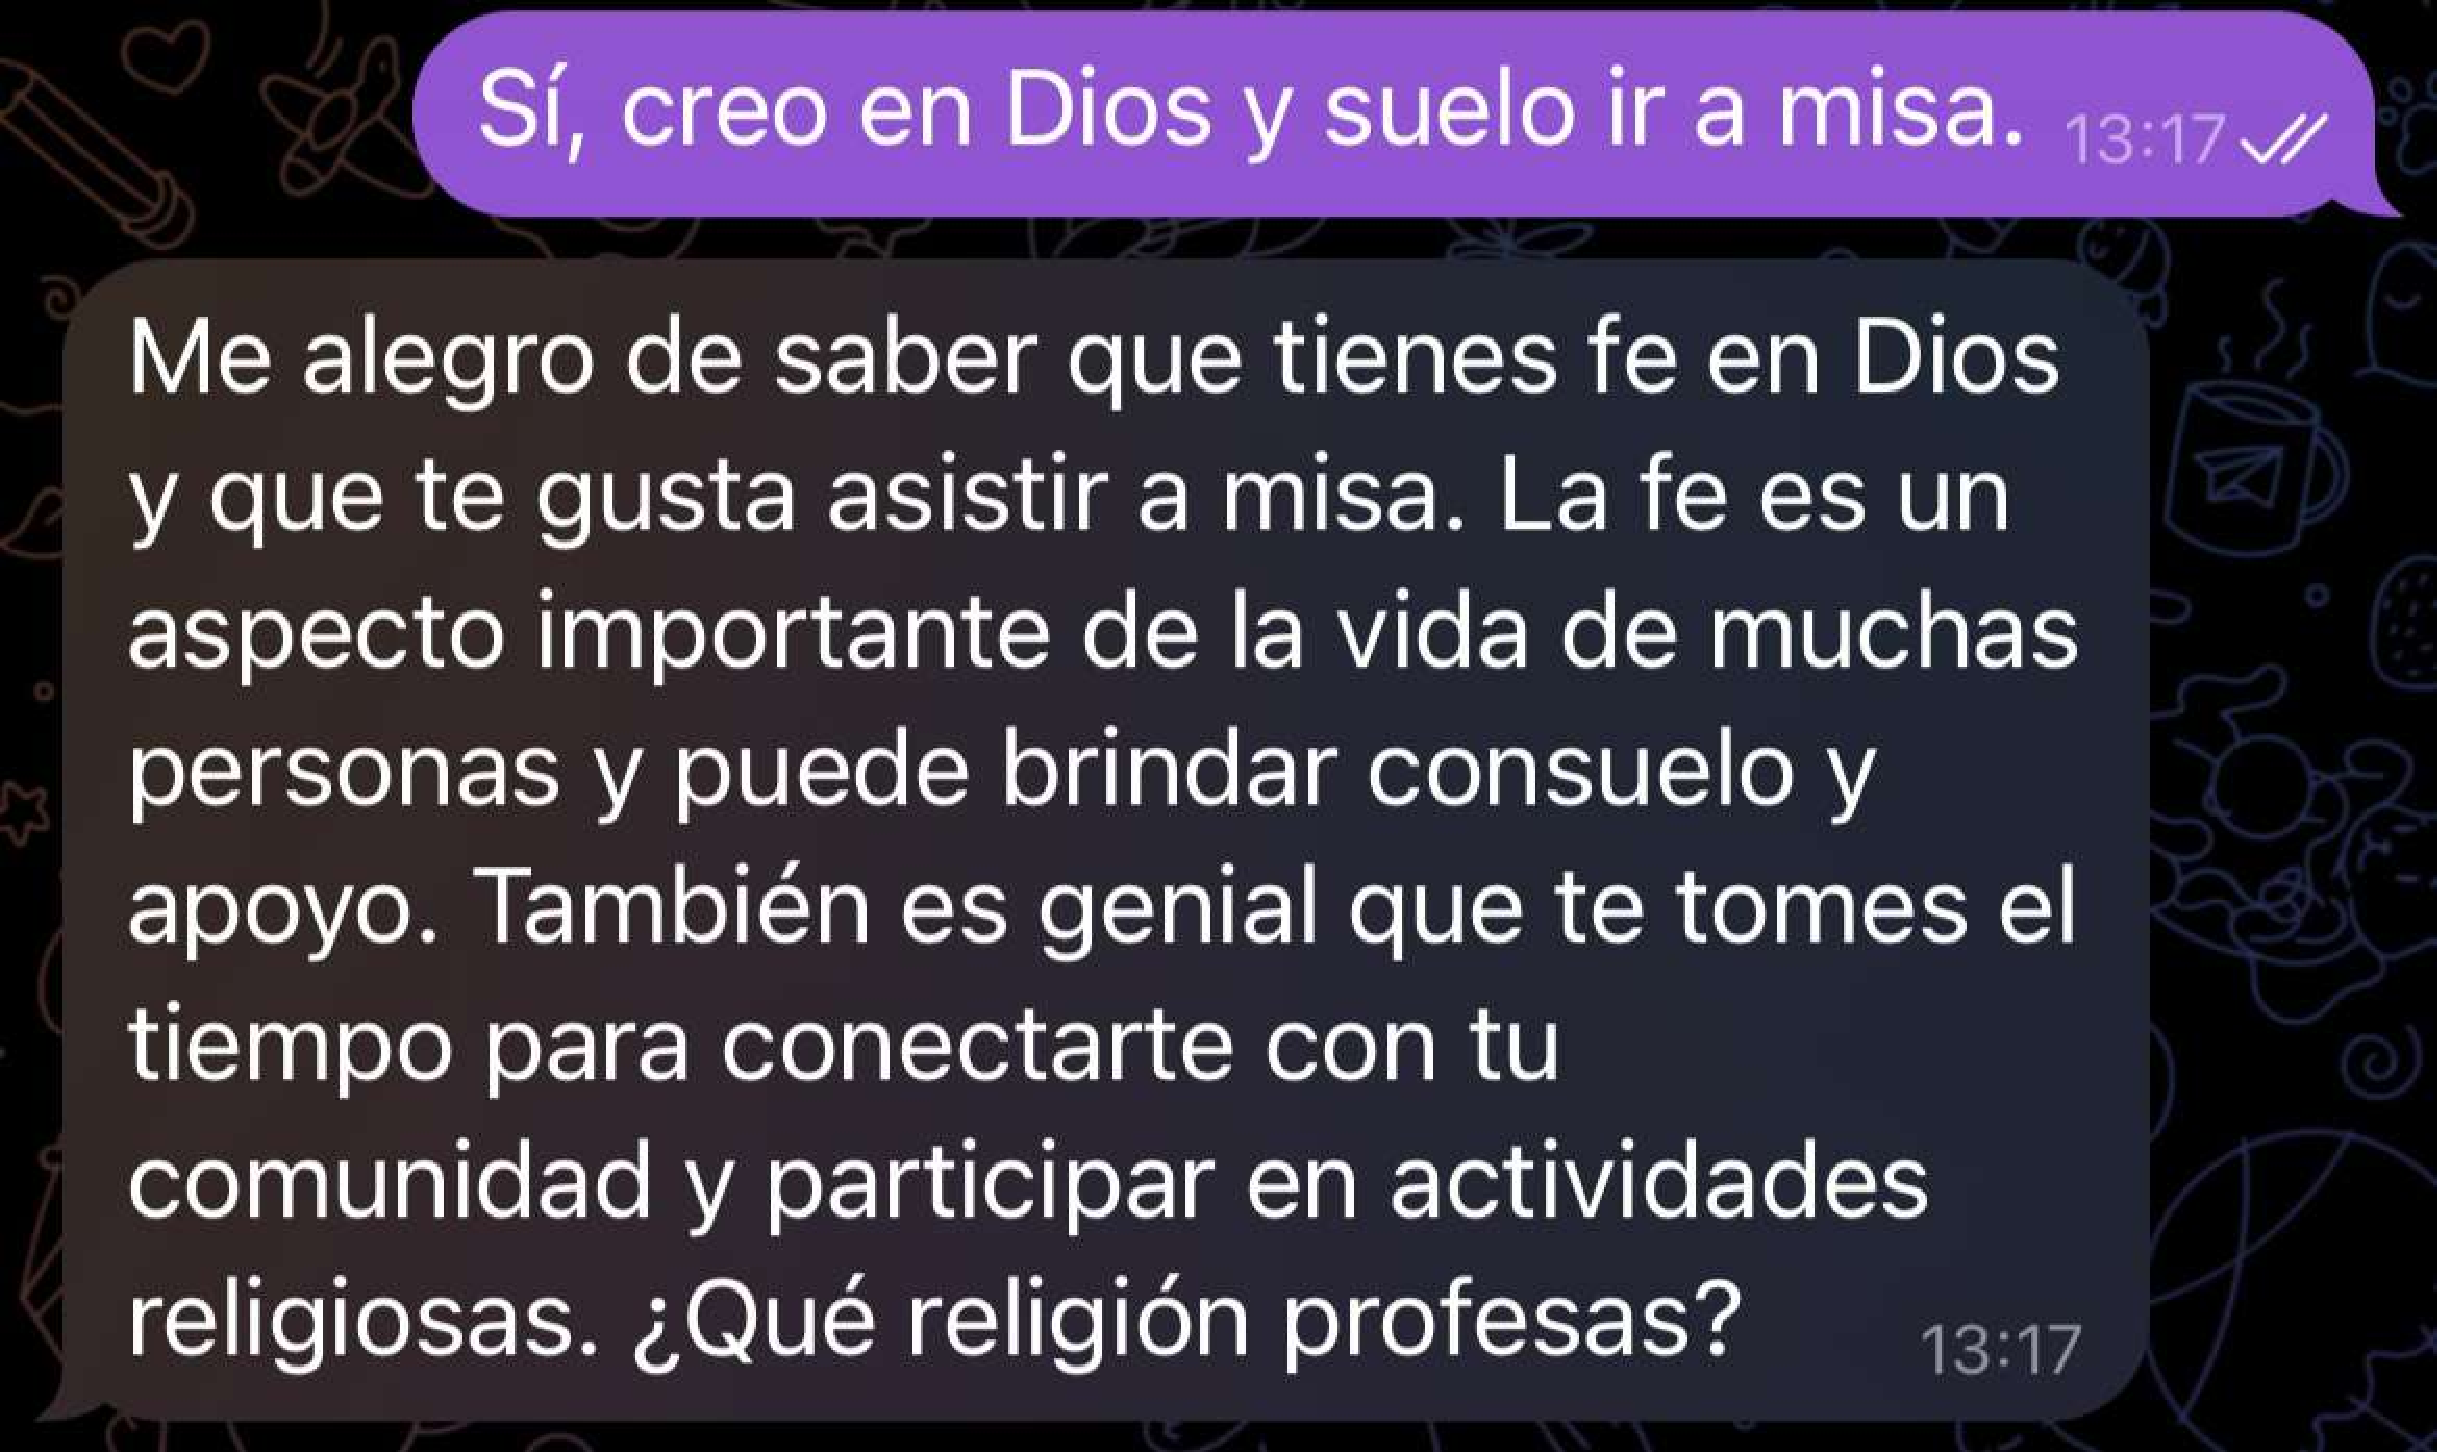
\includegraphics[width=0.6\textwidth]{Imagenes/feedback}
	\caption{Ejemplo de generación de feedback a las respuestas}
	\label{fig:feedback}
\end{figure}


En cualquier momento, una respuesta puede venir acompañada de una imagen y en ese caso, se pasaría al módulo de procesamiento de imagenes.

Recapitulando, el modelo \textit{gemini-pro} se utiliza para las siguientes tareas: 
\begin{itemize}
	\item Análisis de respuestas y transformación de la información extraída a cierto formato que se pueda parsear fácilmente.
	\item Generación de preguntas.
	\item Generación de feedback a las respuestas.
\end{itemize}

Adicionalmente, también se usará para la generación de historias de vida.

\subsubsection{Generación de historias de vida}
Finalmente, se añade la funcionalidad adicional de generar historias de vida. Lo ideal sería generar las historias de vida con otros modelos como el mencionado en \ref{sec:trabajocristina}. Sin embargo, a modo de feedback final de la conversación se propone una historia que podría ser un prototipo de historia de vida. Esta historia es generada por el modelo pasandole un prompt tan simple como el siguiente. 

\begin{verbatim}
	prompt = f"Genera una historia sobre una persona con estos datos
	 {datos}"
\end{verbatim}

La entrada datos, en este caso es un \textit{json} que concatena por cada una de las preguntas los \textit{json} con información que han obtenido. Un ejemplo de generación de historia de vida con este método es la siguiente. 

\begin{verbatim}
	datos = {
		"Nombre": "María",
		"Apodo": "Marucha",
		"Fecha de nacimiento": "15 de febrero de 1930",
		"Lugar de nacimiento": "Barcelona, España",
		"Padres": "Joaquín y Carmen",
		"Hermanos": "Pedro y Ana",
		"Anécdota de infancia": "Una vez me perdí en el parque y un policía 
		me ayudó a encontrar a mis padres.",
		"Mejor amigo de la infancia": "Manuel",
		"Pareja": "Luis, 60 años juntos",
		"Ciudad actual": "Barcelona",
		"Siempre ha vivido en la misma localidad": "Sí",
		"Hijos": "Antonio (60), Marta (58), recuerdo de cuando cocinábamos 
		juntos los domingos.",
		"Nietos": "Carlos (35), Laura (32), recuerdo de las tardes en el parque.",
		"Mascotas": "Rex, perro",
		"Amigos": "Antonio, Rosa",
		"Estudios": "EGB, Bachillerato, Secretariado, diversos cursos de idiomas",
		"Otra cosa que le hubiera gustado estudiar": "Historia del Arte",
		"Anécdota de juventud": "Viajé en tren por toda Europa con mis amigos durante 
		un verano inolvidable.",
		"Ocio en la juventud": "Bailar, tocar el piano",
		"Profesión": "Secretaria",
		"Coches en la vida": "Seat 600, Renault 5",
		"Religiosa": "Sí",
		"Religión": "Católica",
		"Rutinas diarias": "Aseo personal, cuidado de la salud",
		"Deporte de joven": "Natación",
		"Deporte actual": "Paseos diarios",
		"Deporte que le gusta ver": "Tenis",
		"Lectura": "Novelas históricas, periódico local",
		"Programas de televisión": "Concursos y películas",
		"Ir al cine": "Sí",
		"Juegos de mesa": "Cartas y dominó",
		"Aficiones": "Jardinería, pintura",
		"Vacaciones preferidas": "Playa y extranjero",
		"Actividades con pareja": "Viajar y disfrutar de la ópera",
		"Comida favorita": "Paella",
		"Bebida favorita": "Vino tinto",
		"Color favorito": "Azul",
		"Complemento de ropa": "Bufanda",
		"Adornos personales": "Pendientes y pulseras",
		"Relajación": "Estar con familia y escuchar música",
		"Cosas que no soporta": "Ruido excesivo y olores fuertes",
		"Mayor logro en la vida": "Mantener una familia unida",
		"Actividad no realizada que deseaba": "Aprender a bailar flamenco",
		"Actividad que haría de otra manera": "Habría viajado más cuando era joven",
		"Deseo para el resto de su vida": "Seguir disfrutando
		de los momentos con sus seres
		queridos",
		"Deseo por cumplir": "Visitar Japón"
	}
	
	>>>** María: Una vida llena de recuerdos y amor**
	
	María, cariñosamente llamada "Marucha" por su familia, nació un
	soleado 15 de febrero de 1930 en la vibrante ciudad de Barcelona,
	España. Su infancia transcurrió en las calles de la ciudad, donde
	creció rodeada del amor de sus padres, Joaquín y Carmen, y sus dos
	hermanos, Pedro y Ana. 
	
	Un día, mientras jugaba en el parque, la pequeña María se alejó
	demasiado y se perdió. Afortunadamente, un amable policía la
	encontró y la ayudó a regresar con sus padres, quienes la abrazaron
	con alivio y alegría. Este evento quedó grabado en su memoria como
	un recordatorio de la importancia de la familia y la amabilidad
	de los extraños.
	
	Su mejor amigo de la infancia fue Manuel, con quien compartía horas
	de juegos y aventuras. Juntos exploraban la ciudad, descubrían nuevos
	lugares y forjaban una amistad que duraría toda la vida.
	
	En su juventud, María conoció a Luis, el hombre que se convertiría en
	su compañero de vida. Se enamoraron perdidamente y se casaron,
	iniciando un viaje juntos que duraría 60 años llenos de amor, risas
	y complicidad. Formaron una hermosa familia, con dos hijos,
	Antonio y Marta, quienes llenaron su hogar de alegría y bullicio.
	
	
	María siempre había vivido en Barcelona, una ciudad que amaba con
	todo su corazón. Disfrutaba de pasear por sus calles, admirar su
	arquitectura y empaparse de su vibrante cultura. Barcelona era su
	hogar, el lugar donde había vivido toda su vida y donde había
	construido sus más preciados recuerdos.
	
	
	Su vida profesional estuvo marcada por su trabajo como secretaria,
	una profesión que desempeñó con dedicación y responsabilidad. Además
	de su trabajo, María era una mujer apasionada por el aprendizaje.
	Completó sus estudios de EGB y Bachillerato, y luego se
	especializó en Secretariado. Además, siempre mostró interés por
	otros idiomas, tomando diversos cursos para ampliar sus
	conocimientos.
	
	
	Entre sus aficiones favoritas se encontraban la jardinería y la
	pintura. Disfrutaba cuidando de sus plantas y flores, llenando su
	hogar de vida y color. También le encantaba pintar, plasmando en
	sus lienzos los paisajes y momentos que más la inspiraban.
	
	
	Los domingos por la mañana, María y Luis tenían una tradición
	inquebrantable: cocinar juntos. Preparaban deliciosos platos, como
	la paella, su comida favorita, y disfrutaban de largas
	conversaciones mientras compartían la mesa con su familia. Estos
	momentos eran para ella los más preciados, llenos de risas, amor
	y el aroma de la comida casera.
	
	En su tiempo libre, María también disfrutaba de otras actividades
	como leer novelas históricas, ver concursos y películas en la
	televisión, ir al cine, jugar a cartas y dominó con sus amigos
	Antonio y Rosa, y pasear por el parque con sus nietos, Carlos y
	Laura. 
	
	Su fe era una parte importante de su vida. Como católica devota,
	encontraba consuelo y fortaleza en su religión. Las rutinas diarias
	de aseo personal y cuidado de la salud eran esenciales para ella, ya
	que le permitían mantenerse activa y disfrutar de la vida al máximo.
	
	A lo largo de su vida, María ha logrado grandes cosas. El mayor de
	sus logros, sin duda alguna, ha sido mantener una familia unida y
	llena de amor. Ha sido una madre ejemplar, una esposa dedicada y una
	amiga incondicional. A pesar de que tenía algunas actividades
	pendientes, como aprender a bailar flamenco y viajar más cuando era
	joven, no hay duda de que ha vivido una vida plena y feliz.
	
	En la actualidad, María sigue disfrutando de la vida al máximo. Su
	mayor deseo es seguir compartiendo momentos con sus seres queridos y
	atesorando cada instante. También anhela cumplir su último sueño:
	visitar Japón, un país que siempre le ha fascinado.
	
	María es un ejemplo de mujer fuerte, resiliente y llena de amor. Su
	historia es un recordatorio de que la vida es un regalo precioso que
	debemos aprovechar al máximo, llenándola de momentos felices, amor y
	pasión.
	
\end{verbatim}

\subsection{Módulo de procesamiento de imágenes}
\label{procesamientoimagenes}
El módulo de procesamiento de imágenes se encarga de extraer información de las mismas para generar nuevas preguntas y tratar de obtener información adicional. Las imagenes pueden ayudar al paciente a recordar, o expresarse y las preguntas específicas acerca de la imagen son más fáciles de responder que una pregunta genérica sin ningún apoyo visual. 

Una vez llega una imagen al manejador, este la envía apropiadamente a este módulo y a su vez, el módulo llama al modelo  \textit{gemini-pro-vision} para que describa la misma y genere una pregunta. La respuesta a esa pregunta se analizará por el módulo de procesamiento de texto como cualquier otra respuesta. 

Por ejemplo, en la figura \ref{fig:imagenFamilia} vemos un ejemplo de como el chatbot genera información a partir de una imagen y genera una pregunta específica acerca de la imagen. De esta forma, la respuesta asociada a esa pregunta pasa a analizarse como cualquier otra respuesta. 

\begin{figure}[h]
	\centering
	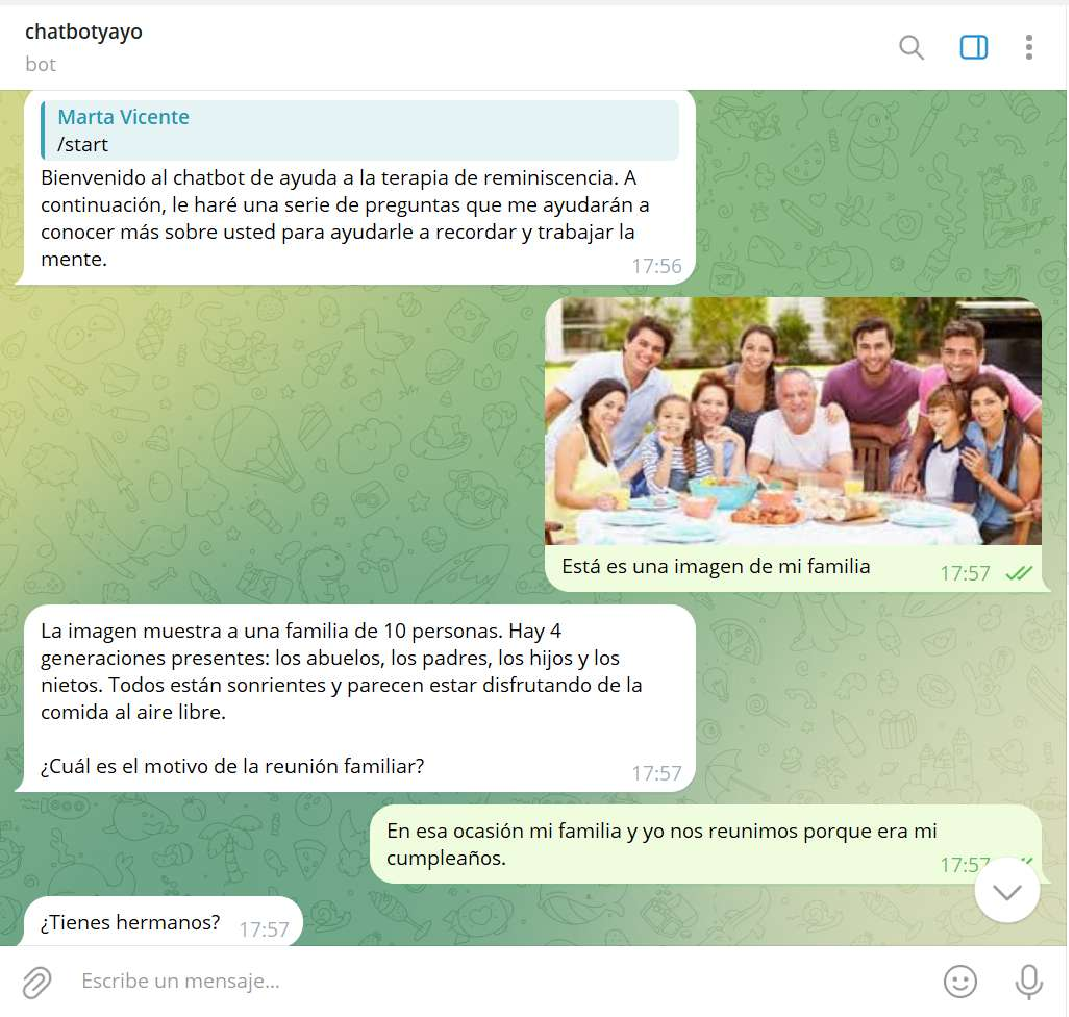
\includegraphics[width=0.9\textwidth]{Imagenes/extracInfoImag}
	\caption{Ejemplo de extracción de información a partir de imagenes}
	\label{fig:imagenFamilia}
\end{figure}

\section{Interfaz e interacción con el usuario}
A pesar de que se podría usar a través de su versión por consola, el chatbot esta pensando para ser usado a través de Telegram. Gracias a esto se puede usar desde tantos dispositivos como se puede usar Telegram, entre los que destacaríamos los dispositivos móviles y los ordenadores.

Para poner en marcha la versión por ordenador, es necesario la aplicación de Telegram, ya sea la versión web o la versión local. De igual forma la versión en móvil u tablet requiere la aplicación de Telegram. Una vez con la aplicación correctamente instalada y abierta, hay que buscar al usuario $\makeatletter @ mavice07\_bot$ y enviado el comando  $\backslash start$, recibiremos el mensaje de bienvenida y comenzará la conversación. Ejemplo de esto en la versión de ordenador y móvil se pueden ver respectivamente en las figuras \ref{fig:bienvenidaOrdenador} y \ref{fig:bienvenidaMovil}.

\begin{figure}[h]
	\centering
	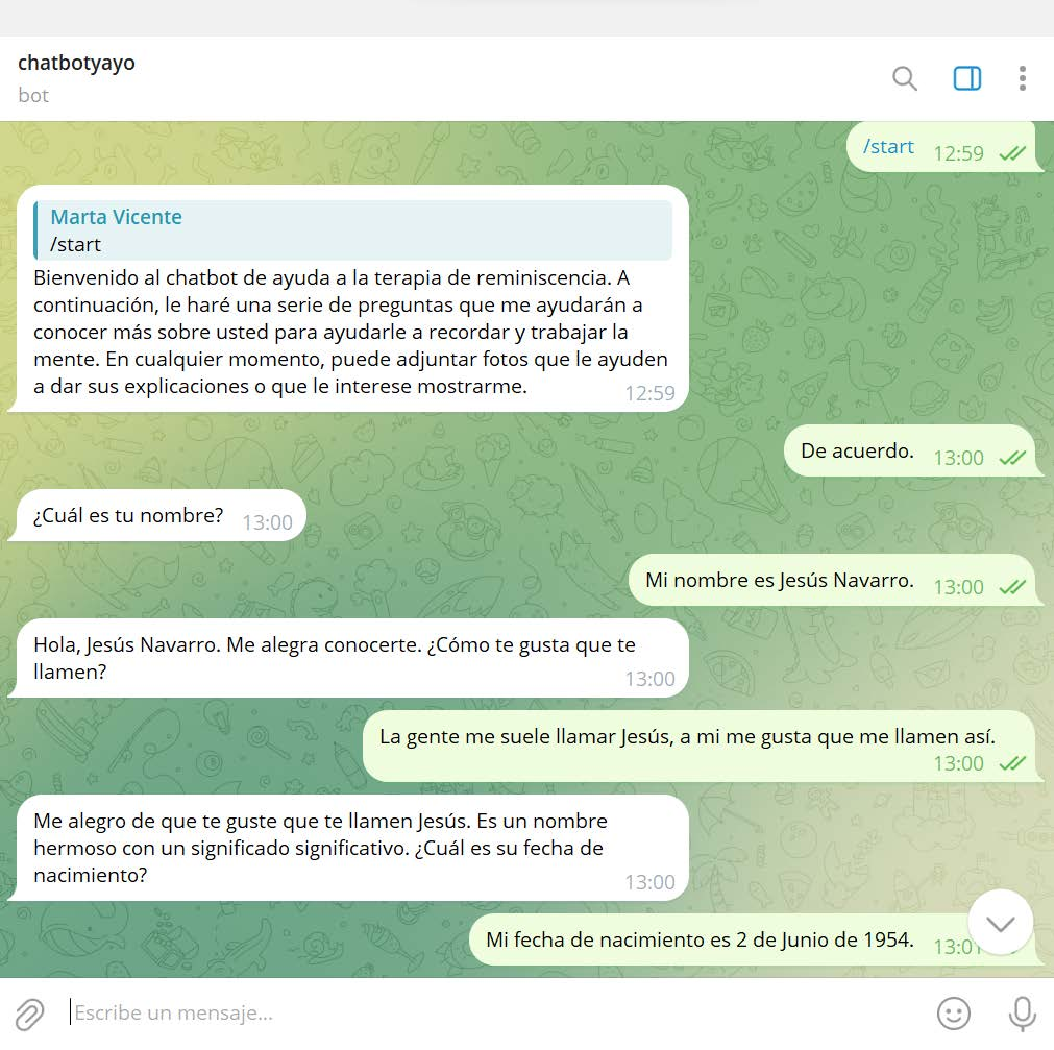
\includegraphics[width=0.8\textwidth]{Imagenes/bienvenidaOrdenador}
	\caption{Ejemplo de bienvenida y primeras interacciones con la versión en ordenador}
	\label{fig:bienvenidaOrdenador}
\end{figure}

\begin{figure}[h]
	\centering
	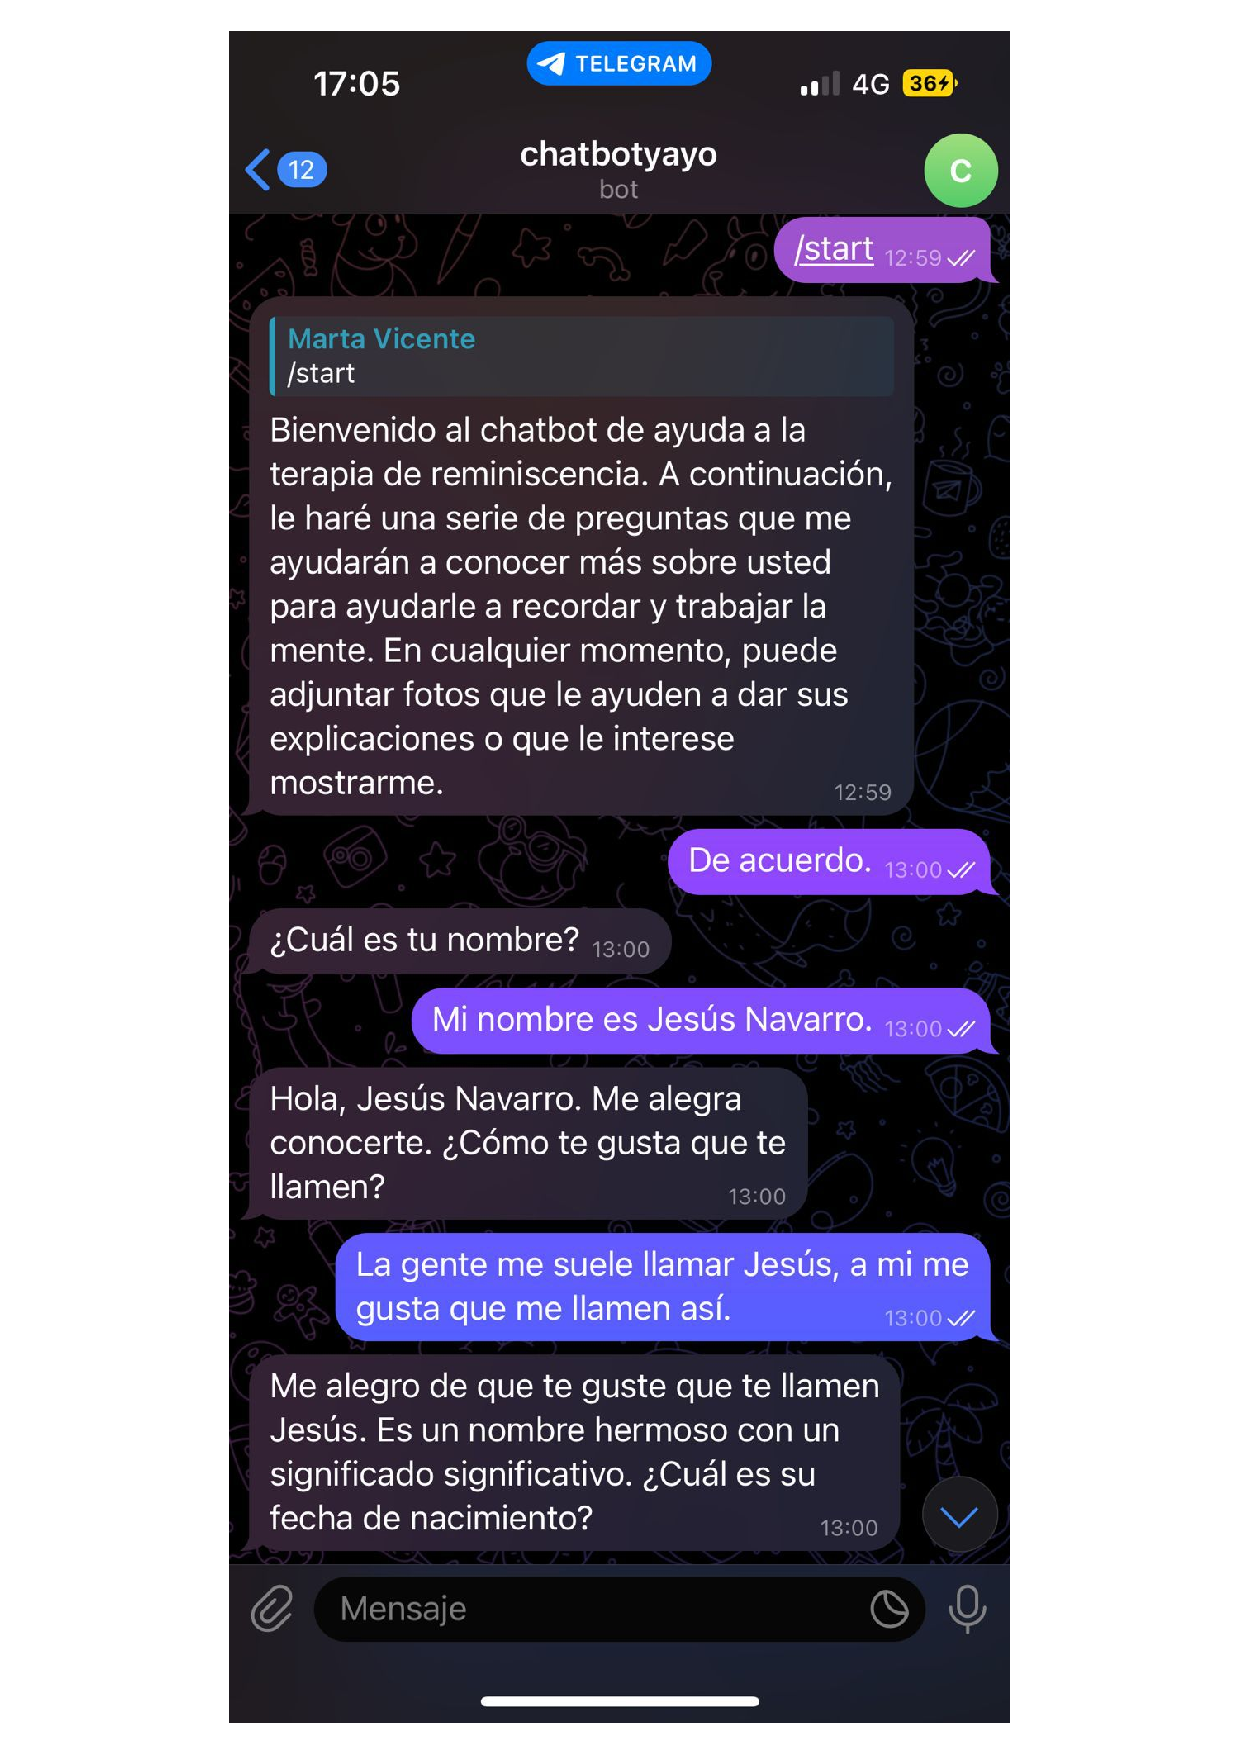
\includegraphics[width=0.8\textwidth]{Imagenes/bienvenidaMovil}
	\caption{Ejemplo de bienvenida y primeras interacciones con la versión en móvil}
	\label{fig:bienvenidaMovil}
\end{figure}





